% Single-cell RNA-seq results (one page). Drop-in: % Single-cell RNA-seq results (one page). Drop-in: % Single-cell RNA-seq results (one page). Drop-in: % Single-cell RNA-seq results (one page). Drop-in: \input{sec_scrna} after the fainter-digits section.
% source: results/scrna/tables.md (verdicts, means over seeds 0-9, alpha grid), prechecks.md; REPORT_scrna.md
% figure: scripts/supervisor_scrna.py
\clearpage
\subsection{Real data: single-cell RNA-seq}
\label{sec:scrna}

\paragraph{Setup.} The cPCA paper's single-cell example \cite{abid2018cpca}, with data from Zheng et al.\ (2017). The target is 7898 bone marrow cells of leukemia (AML) patient 027, 3933 taken before a stem-cell transplant and 3965 after; the background is 1985 cells of a healthy donor. The \emph{signal groups} are the two target samples, pre vs post. The nuisance, shared with the background, is cell type, and was not built to be additive. Preprocessing: log-normalized counts, the 500 most variable genes, each standardized. \methodname{} runs as in \cref{sec:opacity}, without background negatives, on ten seeds, which vary only the algorithms' randomness.

\paragraph{Results} (\cref{fig:scrna} shows seed 0; the claims below use all ten seeds).
\begin{itemize}
  \item \textbf{Accuracy: \methodname{} is the most accurate map, but only by small margins.} It beats every baseline on every seed except t-SNE, where the comparison is not consistent \cpre; apart from cPCA-2D, the gaps are at most 0.02. The 500-gene data already allow 0.951 accuracy, so every map is close to that ceiling and accuracy barely separates the methods \cdesc.
  \item \textbf{Layout: \methodname{} alone places the two samples in two halves of the map,} which is why its ARI is far higher than any baseline's \cdesc. The other maps separate the samples locally but spread both over many cell-type clusters. Plain Neg-t-SNE, the same algorithm on the raw kNN graph, does not produce this layout, so the residual graph is what changes it \cdesc.
  \item \textbf{cPCA:} its label-free rule picks the same $\alpha = 307$ on every seed, a poor choice here. With $\alpha$ chosen using the labels, cPCA$\to$t-SNE becomes slightly more accurate than \methodname{} (0.955 vs 0.944, mean over seeds) \cdesc.
  \item \textbf{Caveats.} Pre and post were sequenced in separate runs at different depths, so part of any separation may be technical, as in the paper's figure; and there is one patient and one donor \cinterp.
\end{itemize}

\begin{figure}[!h]
\centering
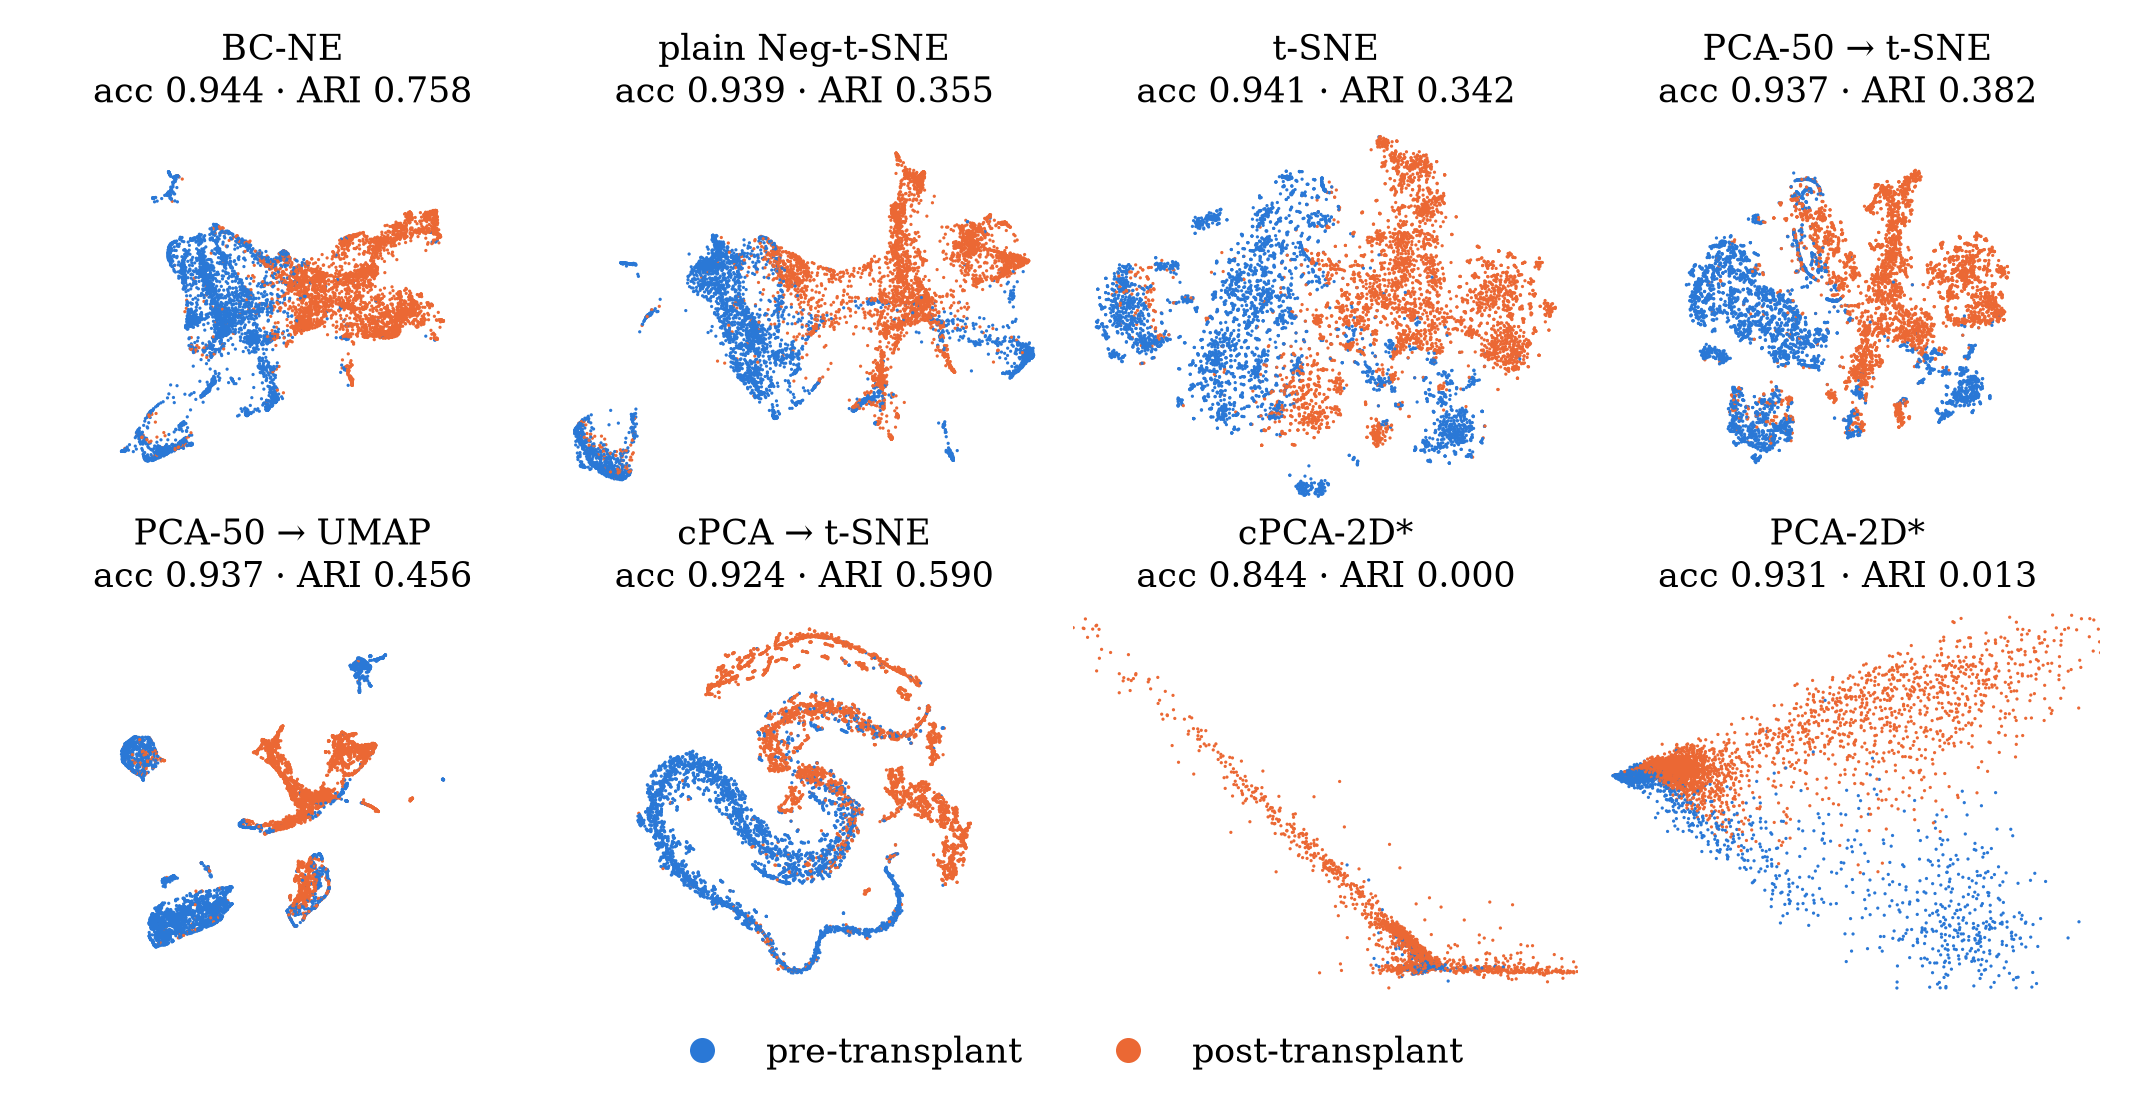
\includegraphics[width=\textwidth]{figures/scrna_seed0.png}
\caption{Single-cell RNA-seq, seed 0, colored by sample, with each map's label kNN accuracy and ARI on this seed. *Drawn on the central 99\% of cells; a few extreme cells otherwise compress these projections to a line.}
\label{fig:scrna}
\end{figure}
 after the fainter-digits section.
% source: results/scrna/tables.md (verdicts, means over seeds 0-9, alpha grid), prechecks.md; REPORT_scrna.md
% figure: scripts/supervisor_scrna.py
\clearpage
\subsection{Real data: single-cell RNA-seq}
\label{sec:scrna}

\paragraph{Setup.} The cPCA paper's single-cell example \cite{abid2018cpca}, with data from Zheng et al.\ (2017). The target is 7898 bone marrow cells of leukemia (AML) patient 027, 3933 taken before a stem-cell transplant and 3965 after; the background is 1985 cells of a healthy donor. The \emph{signal groups} are the two target samples, pre vs post. The nuisance, shared with the background, is cell type, and was not built to be additive. Preprocessing: log-normalized counts, the 500 most variable genes, each standardized. \methodname{} runs as in \cref{sec:opacity}, without background negatives, on ten seeds, which vary only the algorithms' randomness.

\paragraph{Results} (\cref{fig:scrna} shows seed 0; the claims below use all ten seeds).
\begin{itemize}
  \item \textbf{Accuracy: \methodname{} is the most accurate map, but only by small margins.} It beats every baseline on every seed except t-SNE, where the comparison is not consistent \cpre; apart from cPCA-2D, the gaps are at most 0.02. The 500-gene data already allow 0.951 accuracy, so every map is close to that ceiling and accuracy barely separates the methods \cdesc.
  \item \textbf{Layout: \methodname{} alone places the two samples in two halves of the map,} which is why its ARI is far higher than any baseline's \cdesc. The other maps separate the samples locally but spread both over many cell-type clusters. Plain Neg-t-SNE, the same algorithm on the raw kNN graph, does not produce this layout, so the residual graph is what changes it \cdesc.
  \item \textbf{cPCA:} its label-free rule picks the same $\alpha = 307$ on every seed, a poor choice here. With $\alpha$ chosen using the labels, cPCA$\to$t-SNE becomes slightly more accurate than \methodname{} (0.955 vs 0.944, mean over seeds) \cdesc.
  \item \textbf{Caveats.} Pre and post were sequenced in separate runs at different depths, so part of any separation may be technical, as in the paper's figure; and there is one patient and one donor \cinterp.
\end{itemize}

\begin{figure}[!h]
\centering
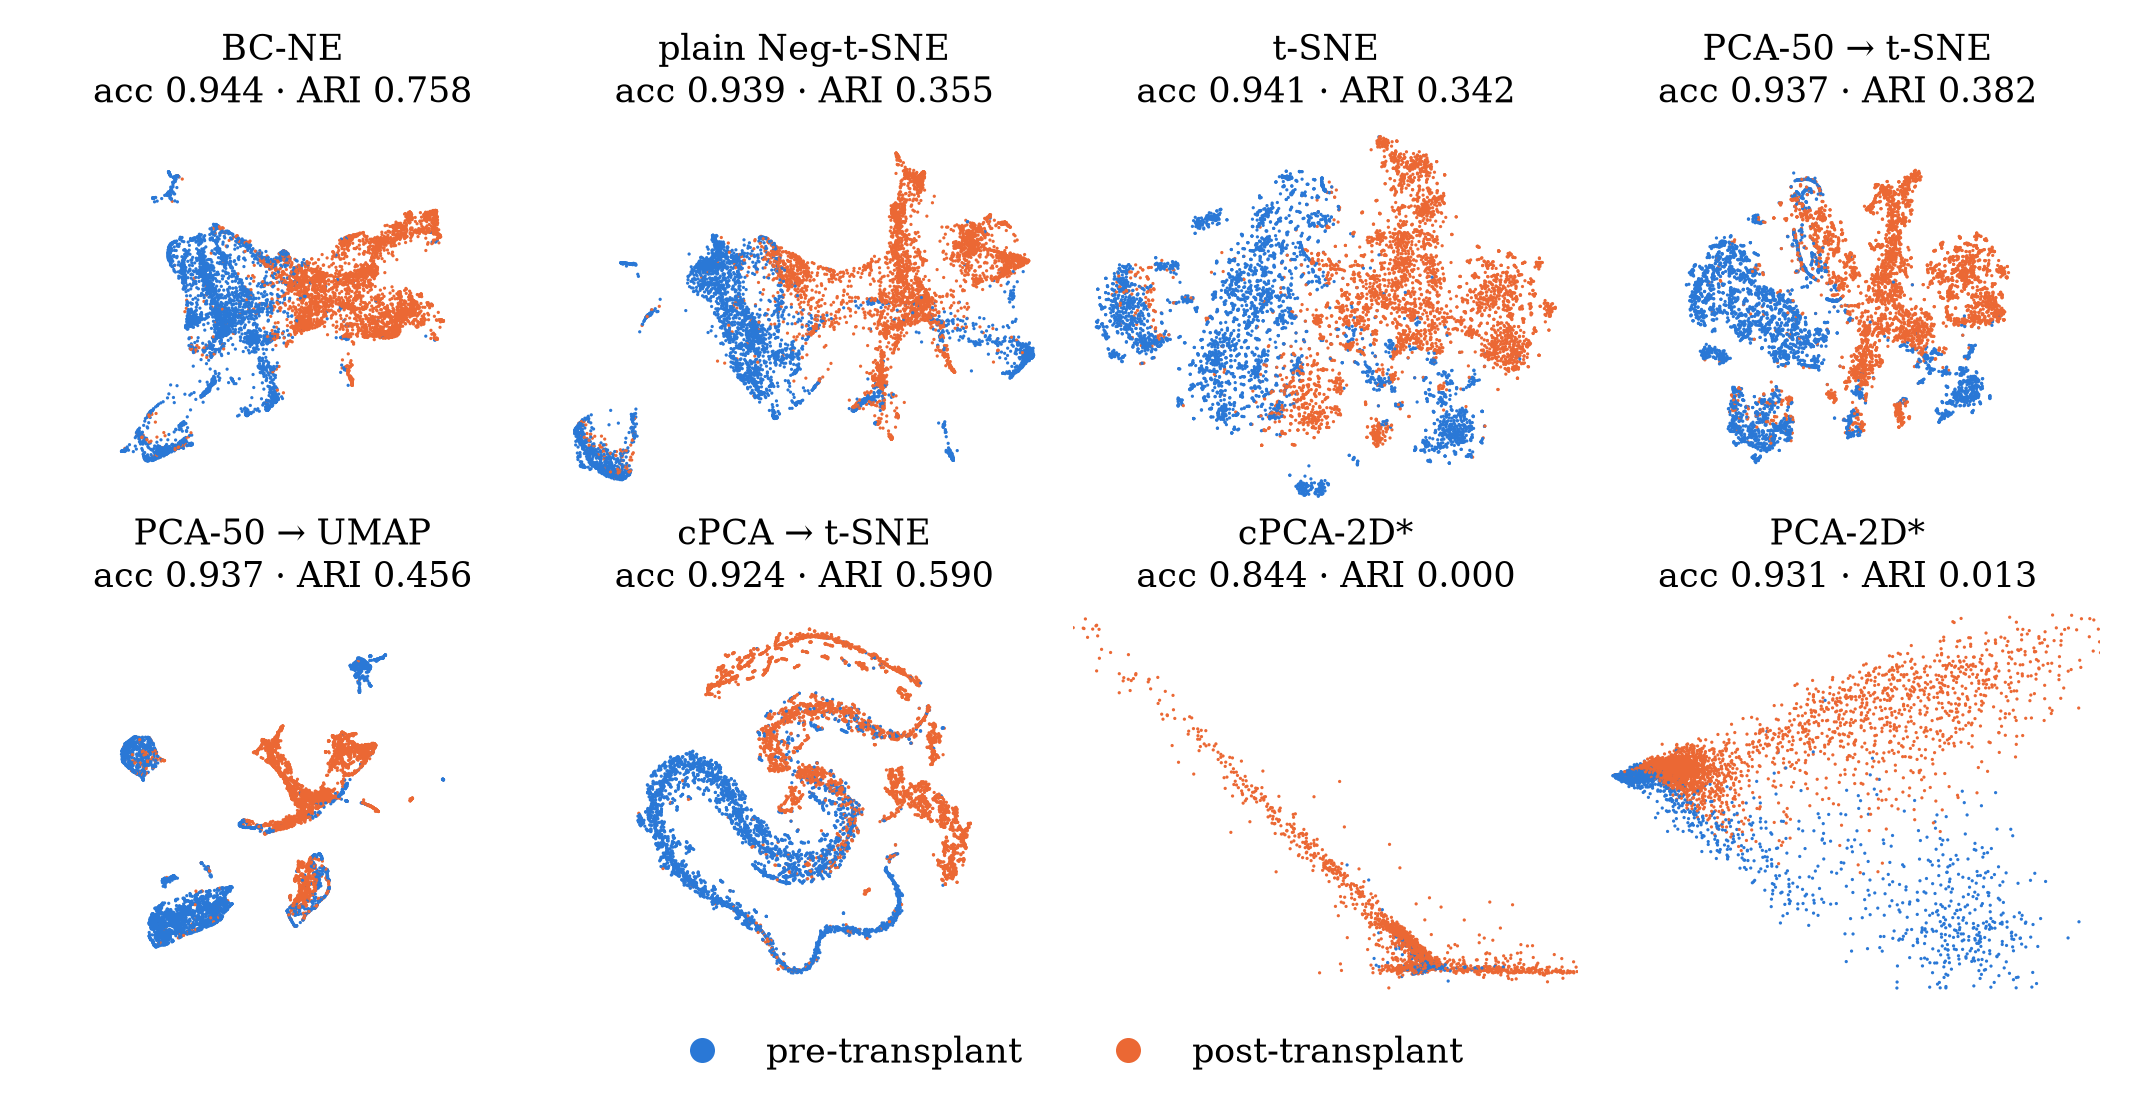
\includegraphics[width=\textwidth]{figures/scrna_seed0.png}
\caption{Single-cell RNA-seq, seed 0, colored by sample, with each map's label kNN accuracy and ARI on this seed. *Drawn on the central 99\% of cells; a few extreme cells otherwise compress these projections to a line.}
\label{fig:scrna}
\end{figure}
 after the fainter-digits section.
% source: results/scrna/tables.md (verdicts, means over seeds 0-9, alpha grid), prechecks.md; REPORT_scrna.md
% figure: scripts/supervisor_scrna.py
\clearpage
\subsection{Real data: single-cell RNA-seq}
\label{sec:scrna}

\paragraph{Setup.} The cPCA paper's single-cell example \cite{abid2018cpca}, with data from Zheng et al.\ (2017). The target is 7898 bone marrow cells of leukemia (AML) patient 027, 3933 taken before a stem-cell transplant and 3965 after; the background is 1985 cells of a healthy donor. The \emph{signal groups} are the two target samples, pre vs post. The nuisance, shared with the background, is cell type, and was not built to be additive. Preprocessing: log-normalized counts, the 500 most variable genes, each standardized. \methodname{} runs as in \cref{sec:opacity}, without background negatives, on ten seeds, which vary only the algorithms' randomness.

\paragraph{Results} (\cref{fig:scrna} shows seed 0; the claims below use all ten seeds).
\begin{itemize}
  \item \textbf{Accuracy: \methodname{} is the most accurate map, but only by small margins.} It beats every baseline on every seed except t-SNE, where the comparison is not consistent \cpre; apart from cPCA-2D, the gaps are at most 0.02. The 500-gene data already allow 0.951 accuracy, so every map is close to that ceiling and accuracy barely separates the methods \cdesc.
  \item \textbf{Layout: \methodname{} alone places the two samples in two halves of the map,} which is why its ARI is far higher than any baseline's \cdesc. The other maps separate the samples locally but spread both over many cell-type clusters. Plain Neg-t-SNE, the same algorithm on the raw kNN graph, does not produce this layout, so the residual graph is what changes it \cdesc.
  \item \textbf{cPCA:} its label-free rule picks the same $\alpha = 307$ on every seed, a poor choice here. With $\alpha$ chosen using the labels, cPCA$\to$t-SNE becomes slightly more accurate than \methodname{} (0.955 vs 0.944, mean over seeds) \cdesc.
  \item \textbf{Caveats.} Pre and post were sequenced in separate runs at different depths, so part of any separation may be technical, as in the paper's figure; and there is one patient and one donor \cinterp.
\end{itemize}

\begin{figure}[!h]
\centering
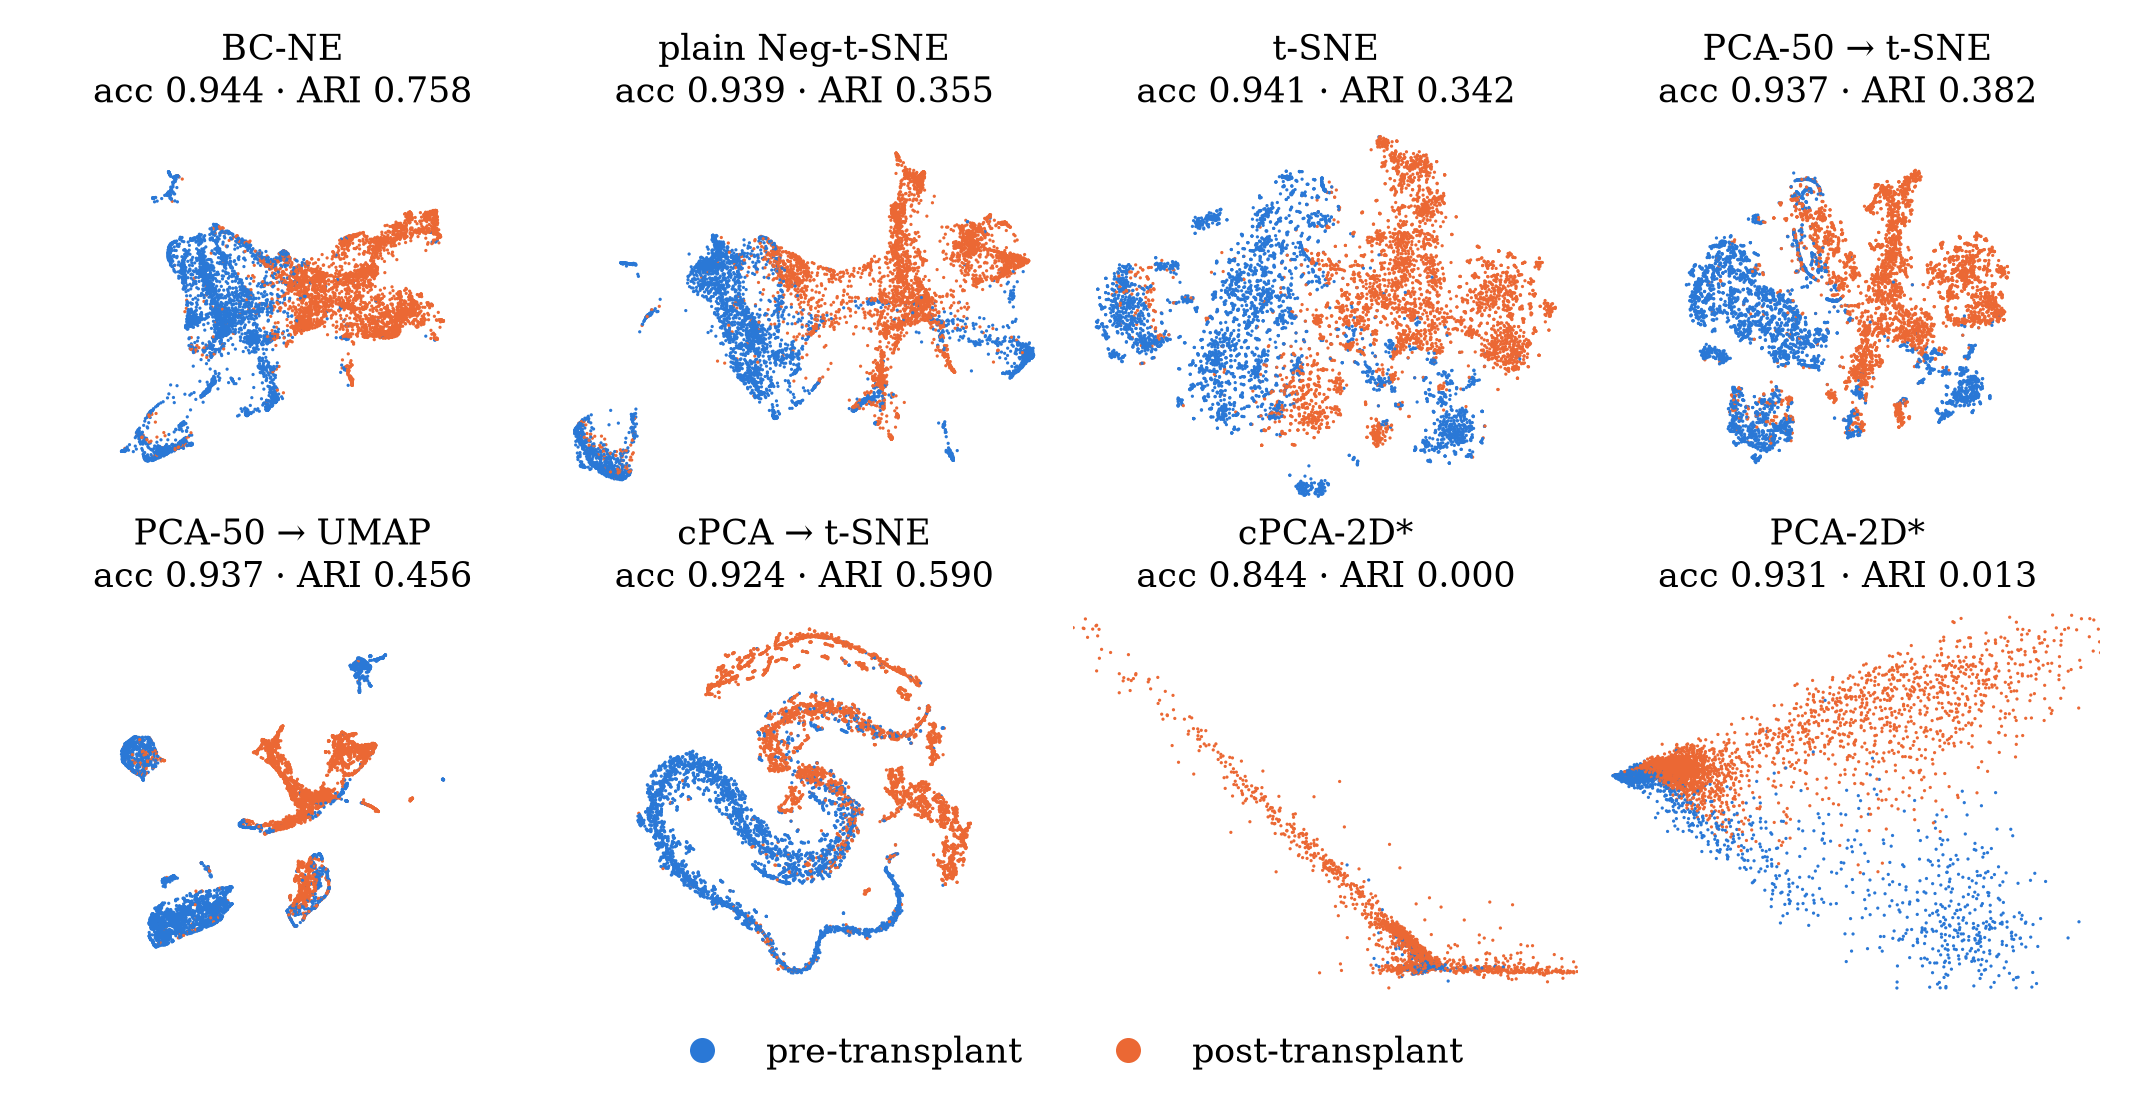
\includegraphics[width=\textwidth]{figures/scrna_seed0.png}
\caption{Single-cell RNA-seq, seed 0, colored by sample, with each map's label kNN accuracy and ARI on this seed. *Drawn on the central 99\% of cells; a few extreme cells otherwise compress these projections to a line.}
\label{fig:scrna}
\end{figure}
 after the fainter-digits section.
% source: results/scrna/tables.md (verdicts, means over seeds 0-9, alpha grid), prechecks.md; REPORT_scrna.md
% figure: scripts/supervisor_scrna.py
\clearpage
\subsection{Real data: single-cell RNA-seq}
\label{sec:scrna}

\paragraph{Setup.} The cPCA paper's single-cell example \cite{abid2018cpca}, with data from Zheng et al.\ (2017). The target is 7898 bone marrow cells of leukemia (AML) patient 027, 3933 taken before a stem-cell transplant and 3965 after; the background is 1985 cells of a healthy donor. The \emph{signal groups} are the two target samples, pre vs post. The nuisance, shared with the background, is cell type, and was not built to be additive. Preprocessing: log-normalized counts, the 500 most variable genes, each standardized. \methodname{} runs as in \cref{sec:opacity}, without background negatives, on ten seeds, which vary only the algorithms' randomness.

\paragraph{Results} (\cref{fig:scrna} shows seed 0; the claims below use all ten seeds).
\begin{itemize}
  \item \textbf{Accuracy: \methodname{} is the most accurate map, but only by small margins.} It beats every baseline on every seed except t-SNE, where the comparison is not consistent \cpre; apart from cPCA-2D, the gaps are at most 0.02. The 500-gene data already allow 0.951 accuracy, so every map is close to that ceiling and accuracy barely separates the methods \cdesc.
  \item \textbf{Layout: \methodname{} alone places the two samples in two halves of the map,} which is why its ARI is far higher than any baseline's \cdesc. The other maps separate the samples locally but spread both over many cell-type clusters. Plain Neg-t-SNE, the same algorithm on the raw kNN graph, does not produce this layout, so the residual graph is what changes it \cdesc.
  \item \textbf{cPCA:} its label-free rule picks the same $\alpha = 307$ on every seed, a poor choice here. With $\alpha$ chosen using the labels, cPCA$\to$t-SNE becomes slightly more accurate than \methodname{} (0.955 vs 0.944, mean over seeds) \cdesc.
  \item \textbf{Caveats.} Pre and post were sequenced in separate runs at different depths, so part of any separation may be technical, as in the paper's figure; and there is one patient and one donor \cinterp.
\end{itemize}

\begin{figure}[!h]
\centering
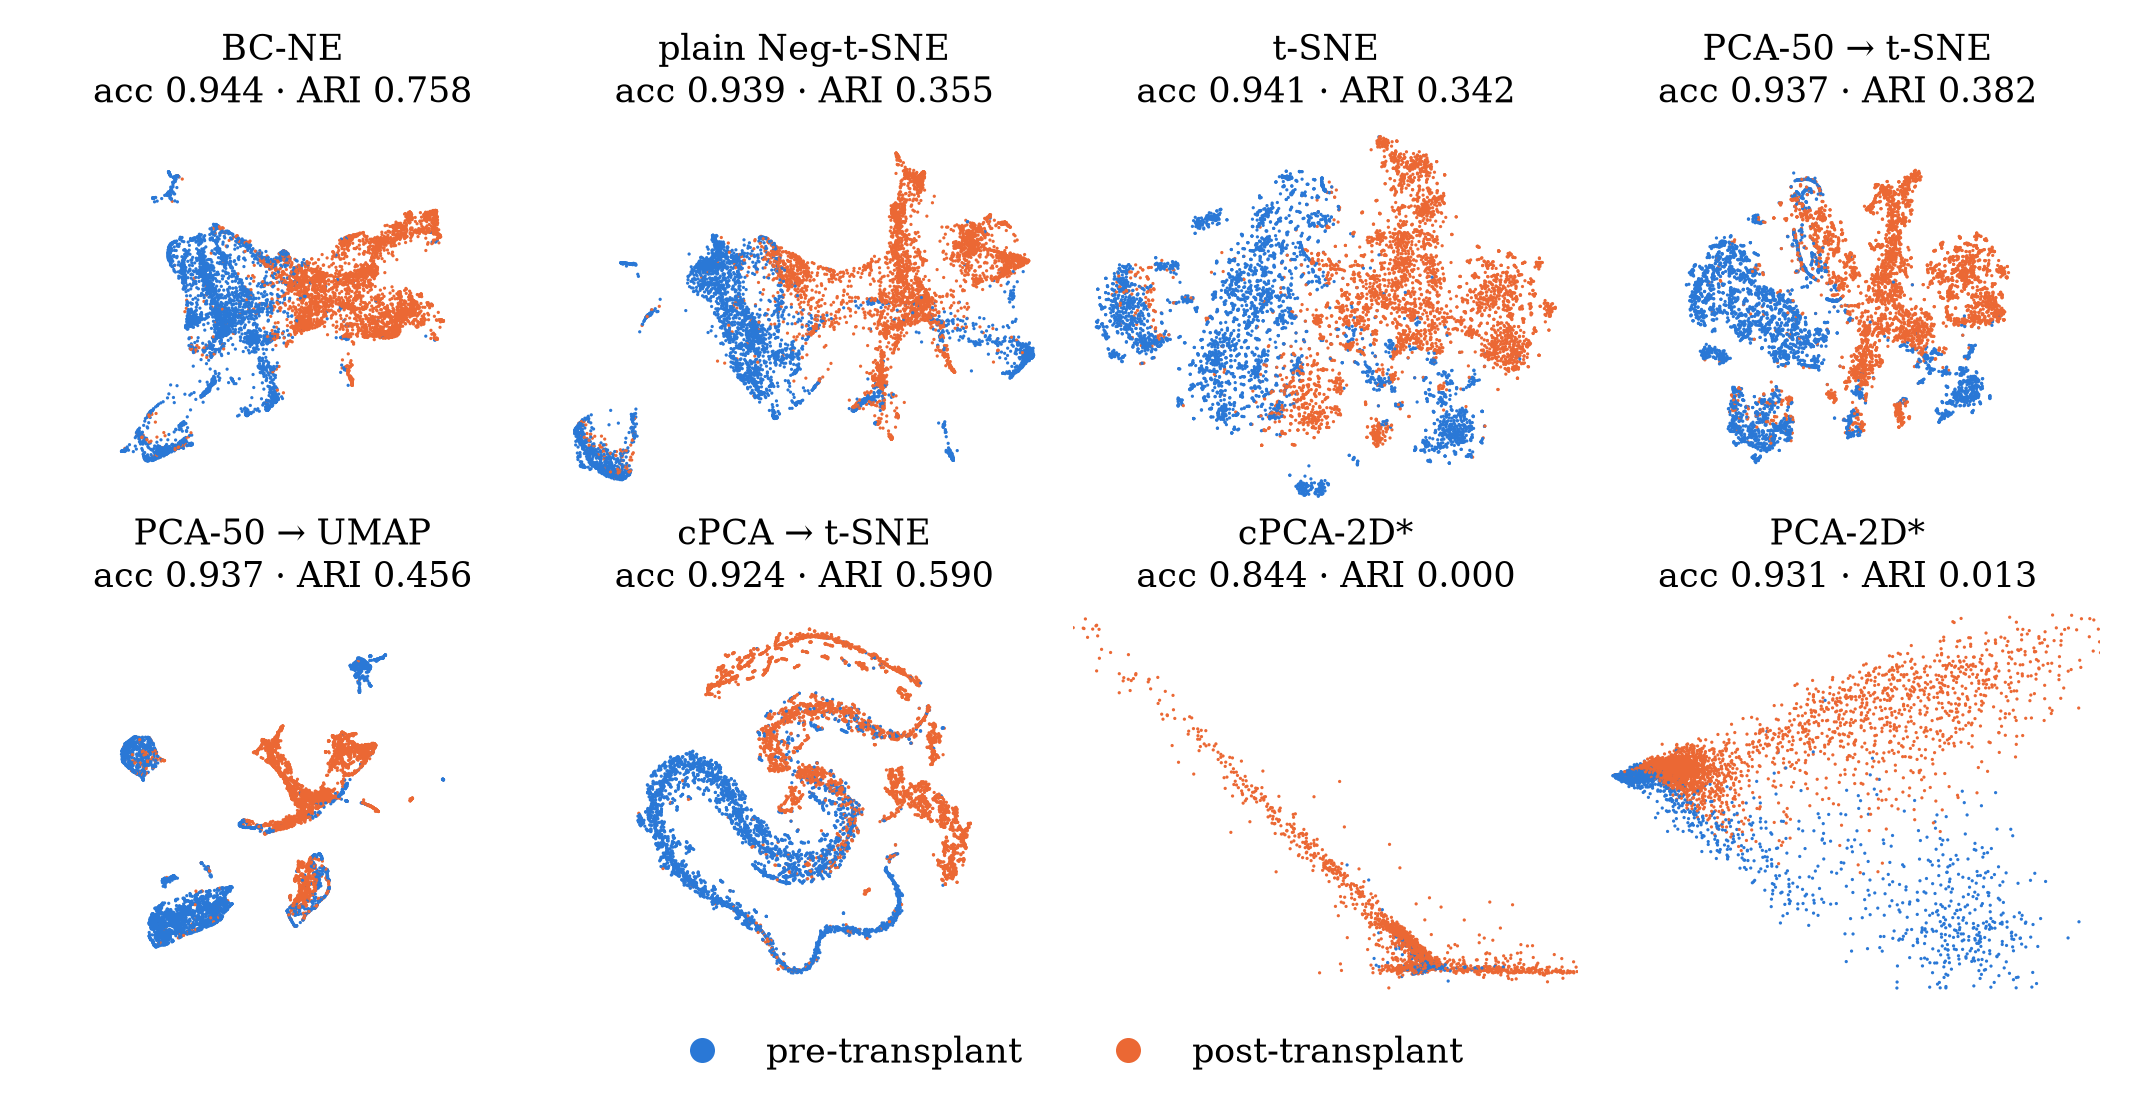
\includegraphics[width=\textwidth]{figures/scrna_seed0.png}
\caption{Single-cell RNA-seq, seed 0, colored by sample, with each map's label kNN accuracy and ARI on this seed. *Drawn on the central 99\% of cells; a few extreme cells otherwise compress these projections to a line.}
\label{fig:scrna}
\end{figure}
